\documentclass[a4paper,12pt]{article}
\usepackage[french]{babel}
\usepackage[utf8x]{inputenc}
\usepackage{amsmath}
\usepackage{graphicx}
\usepackage[colorinlistoftodos]{todonotes}
\usepackage{hyperref}
\usepackage{fullpage}
\usepackage{enumitem}
\usepackage{float}
\usepackage[linesnumbered,ruled,french,onelanguage]{algorithm2e}
\makeatletter 
\g@addto@macro{\@algocf@init}{\SetKwInput{KwOut}{Sortie}}
\makeatother
\usetikzlibrary{arrows}
\usepackage{tikz}
\renewcommand{\baselinestretch}{1.2}
\usepackage[babel=true]{csquotes}
\hypersetup{
	linkcolor=black,
    colorlinks=true,    
    urlcolor=blue,
}

\begin{document}

\begin{titlepage}

\newcommand{\HRule}{\rule{\linewidth}{0.5mm}}

\center
\textsc{\LARGE Université de Caen}\\[1.5cm]
\textsc{\Large Travail Personnel Approfondi}\\[0.5cm]

\textsc{\Large L2 Informatique Groupe 4B}\\[0.5cm]

\HRule \\[0.4cm]
{ \huge \bfseries Projet COREWAR}\\[0.4cm]
\HRule \\[1.5cm]

\begin{minipage}{0.4\textwidth}
\begin{flushleft} \large
\emph{Auteurs :}\\
Robin \textsc{GALLIS}\\
Pierre \textsc{MAURAND}\\
Nicolas \textsc{AUBRY}\\
Thomas \textsc{FILLION}
\end{flushleft}
\end{minipage}
\begin{minipage}{0.4\textwidth}
\begin{flushright} \large
\emph{Professeurs :} \\
Mr Grégory\textsc{ BONNET}\\
Mme Céline\textsc{ ALEC}
\end{flushright}
\end{minipage}\\[2cm]

{\large \today}\\[2cm]

\includegraphics{logo.png}\\[1cm]
\vfill

\end{titlepage}
\tableofcontents{}
\pagebreak
\section{Introduction}
Le \href{https://docs.oracle.com/javase/7/docs/api/}{\underline{Java}} est indéniablement l'un des langages de programmation les plus connus.\\
De part son fonctionnement orienté objet, il était indispensable de nous y attarder et d'en comprendre les subtilités afin de parfaire notre connaissance avancée de la programmation.\\
\indent Afin de réaliser cela, il nous était proposé plusieurs projets en Travail Personnel Approfondi tels que des utilitaires, des jeux vidéos..etc mais parmi tous ses beaux projets, celui qui a le plus retenu notre attention est le \textbf{Projet COREWAR}.\\
L'intitulé de ce projet était :\\
\begin{center}
\enquote{Le but de ce projet est de fournir un outil permettant de générer des programmes efficace au CoreWar. CoreWar est un jeu de programmation dans lequel deux programmes informatiques sont en concurrence pour le contrôle d'une machine virtuelle appelée MARS ( Memory Array Redcode Simulator ). Le but du jeu est de faire se terminer toutes les instances du (ou des) programme(s) adverse(s). Dans un premier temps, il faudra développer une plateforme de simulation de la machine virtuelle (en utilisant une version simple du langage de programmation appelé RedCode).
Dans un second temps, il s'agira d’être capable d’exécuter les programmes écrits en RedCode et de déterminer le vainqueur. Dans la dernière étape, il faudra proposer une méthode (construction
aléatoire, système à base de règles ou encore algorithme génétique) permettant d'obtenir un programme performant.}
\end{center}
\bigbreak
D'après cet énoncé, on peut donc décomposer ce projet en 3 parties:
\begin{center}
\begin{itemize}[label=\textbullet, font=\LARGE]
\item la conception d'une mémoire virtuelle permettant à nos programmes de s'affronter
\item la création d'un interpréteur permettant de lire et comprendre des programmes écrits en RedCode
\item le développement d'un générateur de programmes par le biais d'un "algorithme génétique"
\end{itemize}
\end{center}
\pagebreak
\section{Objectifs du projet}
\subsection{Le CoreWar}
Le CoreWar est un jeu de programmation dans lequel des programmes informatiques sont en concurrence pour le contrôle d'une mémoire virtuelle appelée MARS\footnote{Memory Array RedCode Simulator}. Ces programmes sont écrits dans un langage proche de l'assembleur appelé Redcode. Le but du jeu est donc de détruire tout ses adversaires en terminant leurs instances.
\bigbreak
Comme explicité ci-dessus, le CoreWar interprète du RedCode afin de jouer. Voici le fonctionnement de ce langage :\\
Comme dit précédemment, le RedCode ressemble beaucoup à l'assembleur, de ce fait, un programme jouant sur le coreWar (aussi appelé warrior) sera composé d'une ou plusieurs lignes qui seront sous la forme :\\
\begin{figure}[htpb]
\begin{tikzpicture}
\node[rectangle,rounded corners=5pt,draw] (hot) at (1,1) {Référence};
\node[rectangle,rounded corners=5pt,minimum
size=15pt,draw] (hot) at (2.5,1) {};
\node[rectangle,rounded corners=5pt,draw] (hot) at (4,1) {opération};
\node[rectangle,rounded corners=5pt,minimum
size=15pt,draw] (hot) at (5.5,1) {};
\node[rectangle,rounded corners=5pt,draw] (hot) at (7,1) {mad 1};
\node[rectangle,rounded corners=5pt,draw] (hot) at (8.5,1) {ad 1};
\node[rectangle,rounded corners=5pt,minimum
size=15pt,draw] (hot) at (10,1) {,};
\node[rectangle,rounded corners=5pt,draw] (hot) at (11.5,1) {mad 2};
\node[rectangle,rounded corners=5pt,draw] (hot) at (13,1) {ad 2};
\end{tikzpicture}
\caption{Composition d'une ligne de RedCode normalisée}
\end{figure}\\
\textbf{Référence : }La référence est en quelque sorte une variable qui peut porter n'importe quel nom, et qui va représenter une ligne de telle sorte que cette ligne pourra être appelée plus loin dans le programme afin d'exécuter une nouvelle fois cette ligne avant la fin du cycle\\
\textbf{Opération : }L'opération est l'instruction en RedCode qui va être exécutée par cette ligne\\
\textbf{Mode d'adressage 1(mad 1) : }Il représente la façon dont l'opérande va utiliser la première adresse.\\
\textbf{adressage 1(ad 1):} Cela représente l'endroit dans la mémoire ou l'opérande va chercher l'information dont elle a besoin.\\
\textbf{mode d'adressage 2(mad 2) et adressage 2(ad 2) : }Fonctionnement de la même façon que leurs prédécesseurs a la différence qu'ils ne sont pas tout le temps présents lorsqu'il y a des instructions comme "JMP" par exemple.
\bigbreak
Tout ceci va jouer sur une mémoire de 8000 cases avec un placement aléatoire des warriors sur celle-ci. Chacune des instructions des warriors sera sur une case différentes, toutes à la suite, et un pointeur va avancer petit à petit sur chacune des cases afin d'exécuter l'instruction qui s'y trouve.

\subsection{Notre implémentation : Le NPRT}
Le coreWar n'ayant pas de normalisation précise, et, ayant beaucoup changé en 30ans, nous devions créer notre propre coreWar en s'inspirant de ce qui existait déjà. Pour ce faire, nous nous sommes inspirés du coreWar ICWS’88\footnote{International Core Wars Society}. Voici donc ce à quoi ressemble une ligne en redcode NPRT\footnote{Signifie : Nicolas, Pierre, Robin Thomas} :
\begin{figure}[htpb]
\begin{tikzpicture}
\node[rectangle,rounded corners=5pt,draw] (hot) at (4,1) {opération};
\node[rectangle,rounded corners=5pt,minimum
size=15pt,draw] (hot) at (5.5,1) {};
\node[rectangle,rounded corners=5pt,draw] (hot) at (7,1) {mad 1};
\node[rectangle,rounded corners=5pt,draw] (hot) at (8.5,1) {ad 1};
\node[rectangle,rounded corners=5pt,minimum
size=15pt,draw] (hot) at (10,1) {};
\node[rectangle,rounded corners=5pt,draw] (hot) at (11.5,1) {mad 2};
\node[rectangle,rounded corners=5pt,draw] (hot) at (13,1) {ad 2};
\end{tikzpicture}
\caption{Composition d'une ligne de redcode NPRT}
\end{figure}\\
Pour lister les principales différences, il y a le retrait de la référence, et la séparation entre la première valeur et la deuxième par un simple espace.
\begin{table}[H]
\begin{tabular}{|l|c|c|}
\hline
\textbf{Opération} & ICWS’88 & NPRT \\
\hline
MOV A B : Copie A vers B & x & x \\
\hline
ADD A B : Ajoute A à B & x & x \\
\hline
SUB A B : Soustrait A à B & x & x \\
\hline
JMP A : Saute à l'adresse A & x & x\\
\hline
JMZ A B : Saute à l'adresse A si B est nul & x & x\\
\hline
JMN A B : Saute à l'adresse A si B est non nul & x & x \\
\hline
CMP A B : Si A équivaut à B, saute d'une case & x & x \\
\hline
SLT A B : Si A est inférieur à B, saute d'une case & x & x \\
\hline
DJN A B : Décrémente A, puis saute à l'adresse A si B non nul & x & x \\
\hline
SPL A : Crée un nouvau processus démarrant à l'adresse A & x & x \\
\hline
DAT A : Crée une instruction non exécutable à l'adresse A & x & x \\
\hline
MUL A B : Multiplie A avec B &  & x \\
\hline
DIV A B : Divise A par B &  & x \\
\hline
SEQ A B : Fonctionne comme CMP & & x\\
\hline
SNE A B : Compare A et B et saute une case si ils sont inégaux & & x\\
\hline
MOD A B : Produit la division entière de A par B & & x\\
\hline
DJZ A B : Décrémente A, puis saute à l'adresse A si B nul & & x\\
\hline
\textbf{Type d'adressage} &  &\\
\hline
Vide : Adressage direct & x & x \\
\hline
\#: Adressage immédiat (la valeur est la donnée et l'adresse) & x & x\\
\hline
@ : Adressage indirect (la valeur indique la place dans la mémoire) & x & x\\
\hline
$<$ : Adressage pré-décrémenté (emplacement dans la mémoire de départ) & x & x\\
\hline
$>$ : Adressage post-décrémenté (emplacement dans la mémoire de départ) &  & x\\
\hline

\end{tabular}
\caption{Différence entre notre modèle et le NPRT}
\end{table}
\section{Organisation du projet}
\subsection{Répartition du travail}
Dès la première séance, il a été décidé que nous tiendrons un journal de bord qui est situé \href{https://forge.info.unicaen.fr/projects/core-war/wiki}{ici}. De plus, au vu du travail demandé, nous nous sommes séparés en 2 groupes. Le premier était composé de Nicolas et Robin, et le second était donc composé de Pierre et Thomas. Nicolas et Robin se sont attelés à la réalisation d'un parseur tandis que Pierre et Thomas commençaient à réaliser la mémoire. Le parseur ayant demandé beaucoup moins de temps de réalisation que la mémoire, Nicolas a donc été aider Thomas et Pierre pendant que Robin s'occupait des recherches concernant l'algorithme génétique à réaliser. Parallèlement, Robin réalisait un interpréteur de fichiers et une classe permettant d'écrire dans des fichiers pour pouvoir sauvegarder les nouveaux warriors. Ensuite, après avoir fini le noyau de CoreWar, nous nous sommes tous attelés à la création de l'algorithme génétique. Grâce à une explication complète de cet algorithme par Mr Grégory Bonnet, nous nous sommes séparé en 3. Pierre et Nicolas allaient faire la partie évaluation et sélection de l'algorithme, Thomas quand à lui allait faire la partie mutation de cet algorithme, et pour finir, Robin allait faire la partie population initiale, et la partie reproduction.
\subsection{Architecture}
Concernant l'architecture de notre programme, il est composé de 4 packages qui sont :\\
\begin{center}
\begin{itemize}
\item \textbf{mémoire :} package permettant de gérer la mémoire du CoreWar (placement des warriors, démarrage du combat...etc) ainsi que gérer l'interprétation d'une liste d'instruction donnée(voir ci-dessous).
\item \textbf{interpret :} package permettant de lire des fichiers en ".nprt", de les parser et de les transformer en liste d'instruction afin de les renvoyer à la mémoire. De plus, ce package permet aussi d'écrire une liste d'instruction dans un fichier.
\item \textbf{graphique :} package permettant simplement l'affichage sous forme d'une interface graphique de la mémoire.
\item \textbf{genetics :} package contenant le corps de notre algorithme génétique ainsi que les fichiers ainsi générés.
\pagebreak
\end{itemize}
\end{center}
\begin{figure}[H]
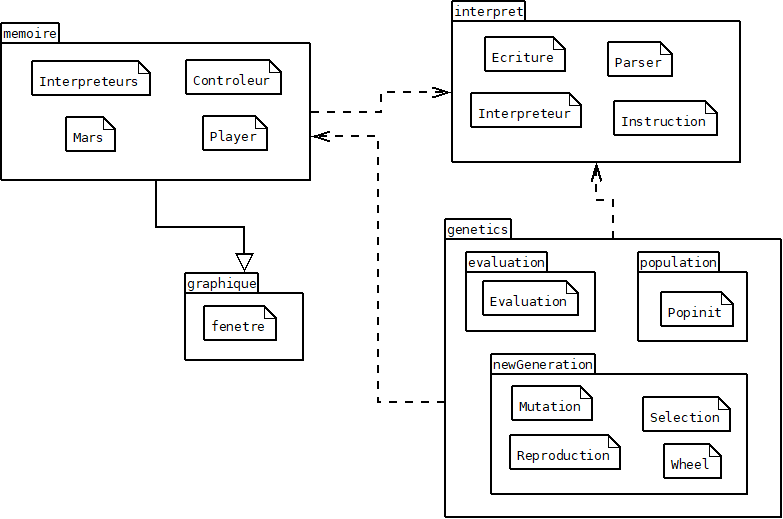
\includegraphics[scale=0.6]{diagrammepackage.png}
\caption{Diagramme de nos packages}
\end{figure}
\begin{figure}[H]
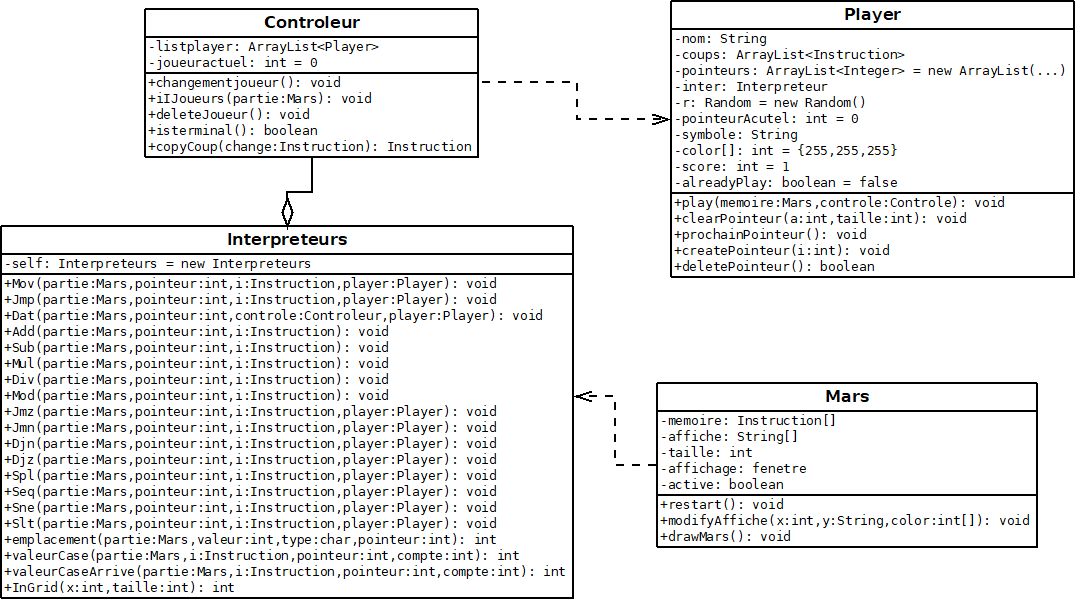
\includegraphics[scale=0.4]{diagrammememoire.png}
\caption{Diagramme de classe du package mémoire}
\end{figure}
\begin{figure}[H]
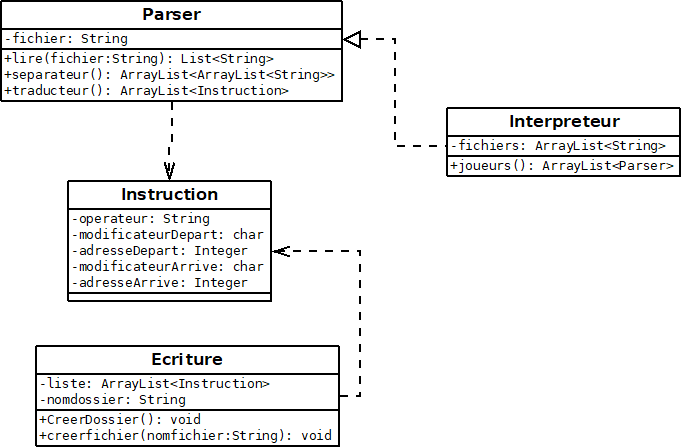
\includegraphics[scale=0.6]{diagrammeinterpret.png}
\caption{Diagramme de classe du package interpret}
\end{figure}
\begin{figure}[H]
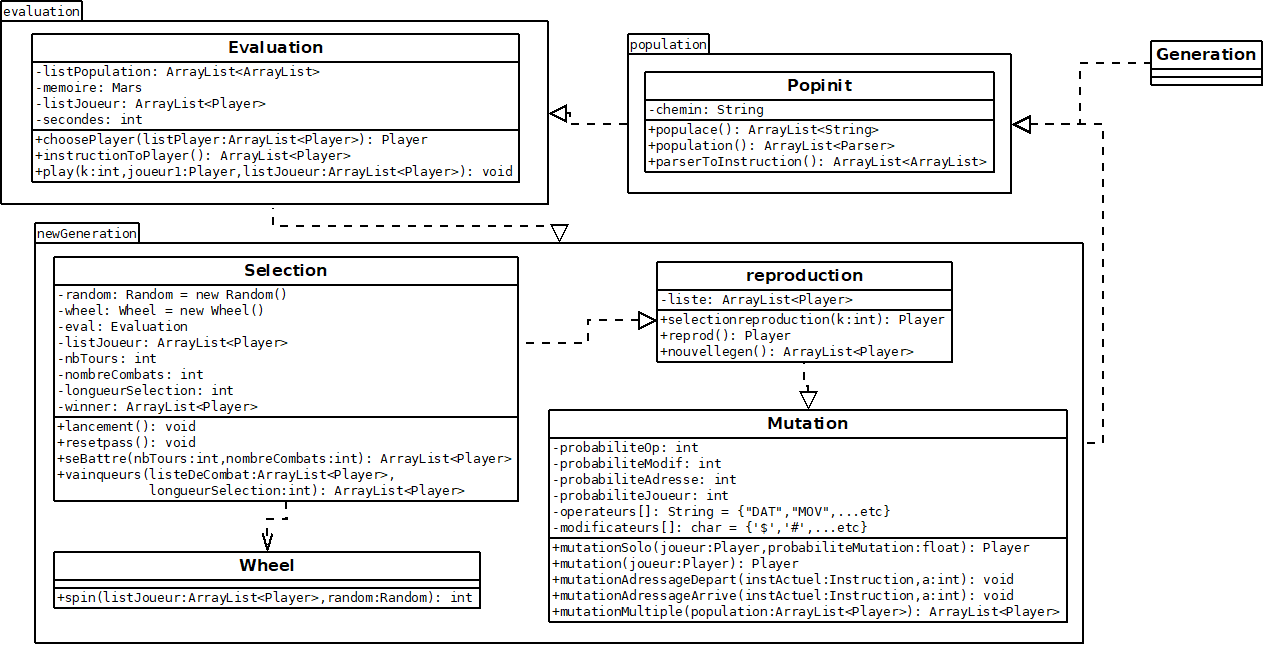
\includegraphics[scale=0.4]{diagrammegenetics.png}
\caption{Diagramme des sous-packages et des classe du package genetics}
\end{figure}
\section{Éléments techniques}
\subsection{La mémoire}
\textbf{MARS:}\\
La classe Mars a pour but de simuler la mémoire d’une machine virtuelle.
Voici à quoi ressemble la mémoire composée de 8100 cases(90*90 cases) :\\
\bigbreak
\begin{figure}[H]
\begin{tikzpicture}
\draw[step=0.7,blue] (0.7,0.7) grid (16.8,1.4);
\node (ff) at (1.05,1.05) {1};
\node (ss) at (16.5,1.05) {8100};
\node (mm) at (8.5,2.05) {Échelle 1/352};
\path[<-,red] (ff) edge[bend right] node[midway,below] {Le pointeur revient au départ} (ss);
\end{tikzpicture}
\caption{Représentation de la mémoire cyclique}
\end{figure}
Initialement remplie d’objets Instructions de type "DAT", elle dispose d’une méthode permettant de modifier son contenu : modifyCase. 
Celle-ci prend en entrée deux arguments, le premier étant la nouvelle Instruction et le second sa position dans la mémoire.
\bigbreak
\textbf{Contrôleur}\\
Quand à elle, la classe Contrôleur s’occupe d'orchestrer la partie. Elle placera premièrement les Instructions des deux joueurs dans la mémoire, puis se chargera du bon déroulement de la partie par exemple en supprimant un joueur quand celui-ci ne possède plus de pointeurs. Enfin, elle a pour rôle d'arrêter la partie quand la mémoire ne possède plus qu’un seul joueur en vie.\\
\textbf{Interpréteur}\\
A l’aide des classes Player, Instruction et Mars, la classe Interpréteur a pour rôle d'interpréter les instances d’instructions. Avec les différents setter et getter de la classe Instruction et de la classe Mémoire, il est aisé d'accéder et de modifier les différentes Instructions dans la mémoire.
\pagebreak

\begin{algorithm}[H]
\DontPrintSemicolon
\KwIn{Une Mars $partie$, un entier $pointeur$,une Instruction $i$ et un Player $player$}
\KwOut{rien}
entier $debut \gets \textbf{emplacement(...)}$\;
Instruction $A \gets \textbf{partie.getcase(debut)}$\;
entier $dest \gets \textbf{emplacement(...)}$\;
modification affichage de la partie\;
modification de la case \;
\caption{{\sc MOV}} 
\end{algorithm}
La fonction "emplacement" appelée dans cet algorithme sert simplement à récupérer la valeur de la case appelée en fonction du mode d'adressage.\\
Toutes les instruction(JMP, ADD...etc) sont basées sur le même modèle que cet algorithme avec les changements qui leurs sont évidemment propres.\\
La classe s'occupe aussi d'interpréter les modificateurs (\$,\#,@,$<$,$>$) pour renvoyer la position brute dans la mémoire. Enfin, elle corrige la position de l'instruction : la mémoire ayant une taille de 8100,si l'instruction doit se placer à la position 8109, la méthode de correction se chargera de remplacer la position par 9.\\
\textbf{Player}\\
Avec sa méthode play, la classe "Player" orchestre le tour d’un joueur, notamment en gérant l'exécution des instructions et l’itérations. 
Aussi elle gère les pointeurs de chaques joueurs.\\
\begin{figure}[H]
\begin{tikzpicture}
\node[rectangle,fill=green,rounded corners=5pt,draw] (hot) at (4,2) {Instruction 1};
\node[rectangle,fill=green,rounded corners=5pt,draw] (hot) at (4,1) {Instruction 2};
\node[rectangle,fill=green,rounded corners=5pt,draw] (hot) at (4,0) {Instruction 3};
\node[rectangle,rounded corners=5pt,draw] (hot) at (4,3) {Liste Instructions Joueur 1};
\node[rectangle,fill=red,rounded corners=5pt,draw] (hot) at (10,2) {Instruction 1};
\node[rectangle,fill=red,rounded corners=5pt,draw] (hot) at (10,1) {Instruction 2};
\node[rectangle,fill=red,rounded corners=5pt,draw] (hot) at (10,0) {Instruction 3};
\node[rectangle,fill=red,rounded corners=5pt,draw] (hot) at (10,-1) {Instruction 4};
\node[rectangle,rounded corners=5pt,draw] (hot) at (10,3) {Liste Instructions Joueur 2};

\node[rectangle,fill=green,rounded corners=5pt,draw] (a) at (0,-2) {Instruction 1};
\node[rectangle,fill=red,rounded corners=5pt,draw] (b) at (3,-2) {Instruction 1};
\path[->,black] (a) edge[bend right] (b);
\node[rectangle,fill=green,rounded corners=5pt,draw] (c) at (6,-2) {Instruction 2};
\path[->,black] (b) edge[bend right] (c);
\node[rectangle,fill=red,rounded corners=5pt,draw] (d) at (9,-2) {Instruction 2};
\path[->,black] (c) edge[bend right] (d);
\node[rectangle,fill=green,rounded corners=5pt,draw] (e) at (12,-2) {Instruction 3};
\path[->,black] (d) edge[bend right] (e);
\node[rectangle,fill=red,rounded corners=5pt,draw] (f) at (12,-4) {Instruction 3};
\path[->,black] (e) edge[bend right] (f);
\node[rectangle,fill=green,rounded corners=5pt,draw] (g) at (9,-4) {Instruction 1};
\path[->,black] (f) edge[bend right] (g);
\node[rectangle,fill=red,rounded corners=5pt,draw] (h) at (6,-4) {Instruction 4};
\path[->,black] (g) edge[bend right] (h);
\end{tikzpicture}
\caption{fonctionnement du déplacement des pointeurs sur les instructions}
\end{figure}
\pagebreak
De part ce fonctionnement, on remarque que à chaque itération, la pointeur va aller se placer en fonction de l'instruction qu'il vient d'exécuter, et, au tour suivant, va exécuter l'instruction située sur la case où il se trouve. Notre schéma représente donc une partie où la case va amener le pointeur sur la case suivante.
\subsection{La gestion de fichiers}
Afin de faciliter la création de warriors ainsi que pouvoir voir l'avancement de notre algorithme par exemple, nous avons mis en place un package permettant la gestion des fichiers (tant dans l'écriture que dans la lecture).\\
\textbf{L'écriture}\\
Afin de pouvoir écrire dans un fichier, nous avons développé une classe nommée "écriture" permettant, comme son nom l'indique, d'écrire dans les fichiers. Cette classe permet, entre autres de créer un fichier qui portera le nom passé en paramètre , ainsi que la création de fichiers multiples via une liste d'instructions, liste qui peut être crée par notre algorithme génétique par exemple. Pour ce faire, on va simplement rediriger la sortie standard vers un fichier créé juste avant.
\bigbreak
\textbf{Le Parseur}\\
Afin de pouvoir exécuter des warriors situés dans des fichiers, il nous fallait construire un parseur qui permettrai de décomposer les lignes des fichiers que nous voulons lire afin de transformer cela en liste d'instructions et ainsi pouvoir jouer avec ce warrior.\\
\begin{algorithm}[H]
\DontPrintSemicolon
\SetKwProg{try}{try}{:}{}
\SetKwProg{catch}{catch}{:}{end}
\KwIn{Un String nommé $fichier$}
\KwOut{Une liste de String contenant toutes les lignes d'un fichier}
File $f \gets new File($fichier$)$\;
Path $lectru \gets Paths.get(Chemin Absolu de f)$\;
Charset $charset \gets Charset.forName("ISO-8859-1")$\;
List$<$String$>$ $lines \gets null$\;
\try{}{
$lines \gets File.readAllLines(lectru, charset)$
}
\catch{IOException e}{
$Afficher \gets e$
}
\uIf{lines.size()$>$50}{
    \Return null \;
}
\Return lines
\caption{{\sc Lecture des lignes d'un fichier}} 

\end{algorithm}

\pagebreak
Ensuite, on va séparer les informations de chaque lignes en considérant qu'un espace signifie que l'information est finie. Et enfin on va créer les liste d'instruction avec notamment la classe Interpreteur.\\
\textbf{L'instruction}\\
L'instruction dont on parle depuis le début nous sert à conserver les informations de  chaque ligne d'un warrior afin de pouvoir les restituer à la mémoire. Nous ne la détaillerons pas car il ne s'agit que d'une simple encapsulation.\\

\subsection{L'algorithme génétique}
\begin{center}
\begin{figure}[H]
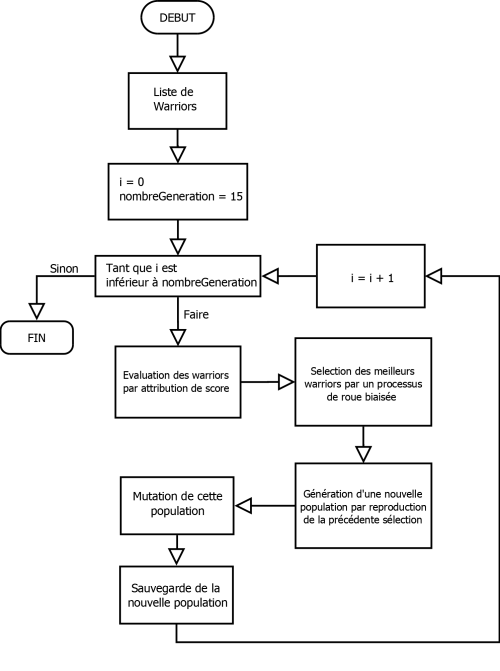
\includegraphics[scale=0.6]{toma.png}
\caption{Algorigramme de l'algorithme génétique}
\end{figure}
\end{center}
\textbf{La population initiale}\\
Dans un algorithme génétique, la population initiale est importante car c'est celle-ci qui va déterminer ce à quoi va ressembler notre nouvelle génération de warriors. En effet, le warrior généré sera bon contre ses parents ,mais pas forcément bon si on choisit une autre population initiale. En soit, l'algorithme génétique va forcément donner un bon warrior localement. En partant de ce postulat, nous avons donc choisit comme population initiale 50 warriors fonctionnels inventés ou repris parmi les warriors qui ont participé aux compétitions mondiale de CoreWar. Afin de récupérer tout ces warriors, nous avons mis en place un sous-package composé de la classe "PopInit".Cette classe permet la récupération et la transformation en liste d'instruction de tout les fichiers présents dans le dossier cible.
\bigbreak
\textbf{L'évaluation}\\
Maintenant que nous avons une population initiale, il nous faut évaluer chacun des programmes afin de pouvoir avoir une référence sur la force de chacun des warriors. Afin de faire une évaluation la plus impartiale possible, nous faisons jouer chacun des warriors contenus dans la population initiale contre 3 autres warriors (valeur modifiable dans les paramètres) choisis aléatoirement. À la suite de chaque combat, un nombre de points seront attribués au joueur qui joue contre les joueurs aléatoires. La note varie entre 8100(Victoire) Et 1 (défaite), les matchs durent un temps modifiable, mais nous avons pour le moment mis des maths de 10 secondes maximum, de ce fait , si au bout des 10 secondes réglementaires aucun gagnant n'est ressorti, on va attribuer au joueur un nombre de points équivalents au nombre de cases possédées. De ce fait, notre algorithme génétique va générer des warriors qui gagnent vite ou qui prennent beaucoup de place dans la mémoire, mais des warriors tels que le "willy" qui peut gagner sûr le long terme seront mal notés.
\bigbreak
\textbf{La nouvelle génération}\\
Afin de créer la nouvelle génération, nous allons devoir passer par 3 étapes :
\begin{itemize}
\item La sélection
\item La reproduction
\item La mutation
\end{itemize}
Après avoir noté chacun des programmes, nous allons pouvoir sélectionner ceux qui vont pouvoir subsister dans la prochaine génération.\\
Pour ceci, 3 choix s'offraient à nous, nous nous sommes intéressés à l'algorithme K-Tournois ainsi qu'à l'algorithme de la roue Biaisée. Après de mures réflexions nous avons choisis la roue biaisée car l'algorithme des K-tournois nous amènerait trop rapidement vers des maximum locaux.\\
Cette roue biaisée va, comme son nom l'indique, avoir plus de chance de sélectionner les warriors qui ont eu plus de points lors de l'évaluation sans pour autant empêcher un warrior potentiellement "nul" d'être sélectionnée.\\
Ensuite vient la reproduction.\\
Pour la reproduction, on va sélectionner 2 warriors aléatoirement, puis il y aura une chance sur 2 que :\\
\begin{itemize}
\item On prenne la moitié de chacun des programmes et on les fusionne
\item On prenne 1/4 du premier programme et  3/4 du deuxième programme et on les fusionne
\end{itemize}
Puis on exécute cette reproduction 25 fois, pour constituer, avec les ressortissants de la roux biaisée, la nouvelle population de 50 warriors.\\
Pour finir, on va appliquer une mutation sur les 50 warriors.\\
Cette dernière étape change très légèrement les Instructions d’une population afin de la rendre de plus en performante au fur et à mesure du temps.

Pour des besoin d'expérimentations, les probabilités de mutation sont à définir lors de la création de l'objet qui instancie la classe. 

Une fois créé, deux méthodes sont à disposition : mutationMultiple et mutationSolo. 
La première prends en entrée une liste de joueur et les faits tous muter avec les mêmes probabilités, la seconde prend en entrée un joueur et une probabilité de mutation initiale ( appel de sous-methode ou non ). 

Cela permet d'appliquer une mutation différente en fonction du score renvoyé par la fonction d'évaluation.

Pour clarifier, les warriors les plus puissants auraient une probabilité anodine de muter tandis que les warriors les plus faibles, une probabilité élevé. Tout cela dans un but d'évolution plus rapide et moins dangereuse pour les têtes de classements.
Cependant, même si la méthode MutationSolo n'est pas plus coûteuse, il est plus coûteux pour l'algorithme génétique de traiter les cas un par un.\\
\begin{algorithm}[H]
\DontPrintSemicolon
\KwIn{Un joueur avec une liste d'instruction $\langle inst_1, inst_2, \ldots, inst_n \rangle$
Des probabilités prédéfinis $\langle prob_1, prob_2,prob_3 \rangle$}
\KwOut{Un joueur avec une nouvelle liste d'instructions, possiblement les mêmes}
$listInstruction \gets \textbf{ Instructions du joueur}$;
$newListInstruction \gets \textbf{ nouvelle liste vide}$;

\For{$instruction \textbf{ in } listInstruction$}{

    $random1 \gets \textbf{ un nombre tiré entre 1 et 10000 }$;

    \If{$random1 < prob_1$}{
        $instruction \gets \textbf{changement de modificateur}$;
    }

    $random2 \gets \textbf{ un nombre tiré entre 1 et 10000 }$;

    \If{$random2 < prob_2$}{
        $instruction \gets \textbf{ +1 ou -1 à l'adressage}$;
    }

    $random3 \gets \textbf{ un nombre tiré entre 1 et 10000}$;

    \If{$random3 < prob_3$}{
        $instruction \gets \textbf{ changement d'operateur}$;
    }

    $newListInstruction\textbf{.ajouter(}instruction\textbf{)}$;
}

$joueur2 \gets \textbf{nouveau joueur avec newListInstruction}$;

\Return{joueur2};
\caption{{\sc mutation}}
\label{algo:mutation} 
\end{algorithm}
\pagebreak
\section{Expérimentations et Usages}
\subsection{La génération du warrior}
Grâce à notre algorithme génétique, nous pouvons dès lors générer une population de warriors, reste maintenant à choisir les bons paramètres afin de générer une population efficace. Nous allons considérer que un warrior est efficace lorsqu'il ne se suicide pas dès le début et qu'il se bat au moins un petit peu.\\
Nous avons donc tentés beaucoup de générations plus ou moins longues.\\
Pour commencer, nous avons tentés une génération avec des combats de 30 seconde, et sur 50 générations. De plus nous avions mis un taux de mutation de 10\%. Cette génération fût infructueuse car, le taux de mutation était beaucoup trop grand, et le nombre de générations lui aussi trop grand.\\
Puis nous avons donc retentés avec cette fois , 15 générations et un taux de mutations de 1\% et par manque de temps des combats de 10 secondes maximum. Cela a été fructueux, les warriors générés marchaient.\\
Pour faire un petit point sur les performances, en lors du premier test, l'algorithme a mis 1h35 à tout générer, tandis que lors du deuxième test il a mis seulement 23 minutes. Ceci est normal car le nombre de générations et la durée des combats ont étés largement réduits. 
\begin{figure}[H]
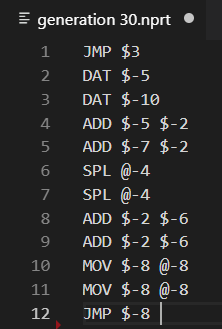
\includegraphics[scale=1]{warior.png}
\caption{L'un de nos warriors générés}
\end{figure}

\subsection{Utilisation du programme}
\begin{figure}[H]
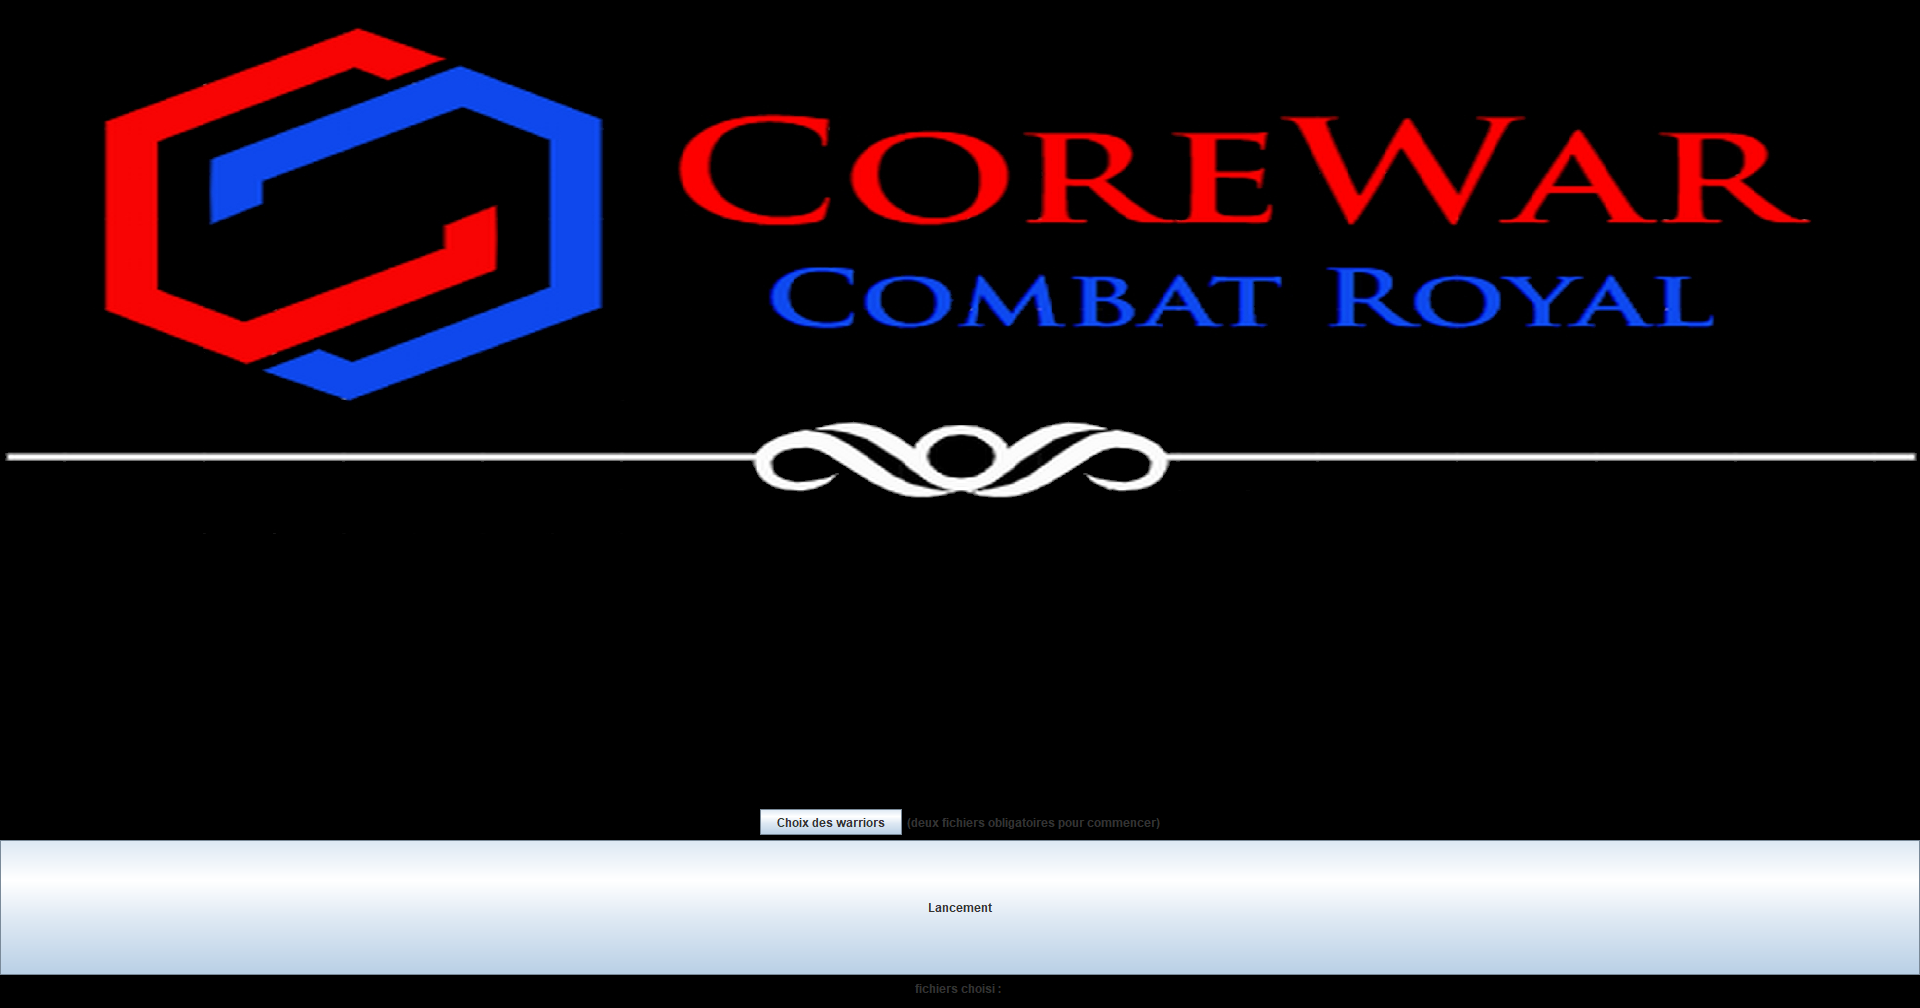
\includegraphics[scale=0.3]{ac.png}
\caption{page d'accueil du coreWar}
\end{figure}
Sur notre page d'accueil, il vous est demandé de choisir deux warriors minimum afin de commencer une partie, ce choix de warriors doit être effectué parmi les warriors situés dans le dossier ("fichiers"). Ensuite vous pourrez commencer la partie.\\
\begin{figure}[H]
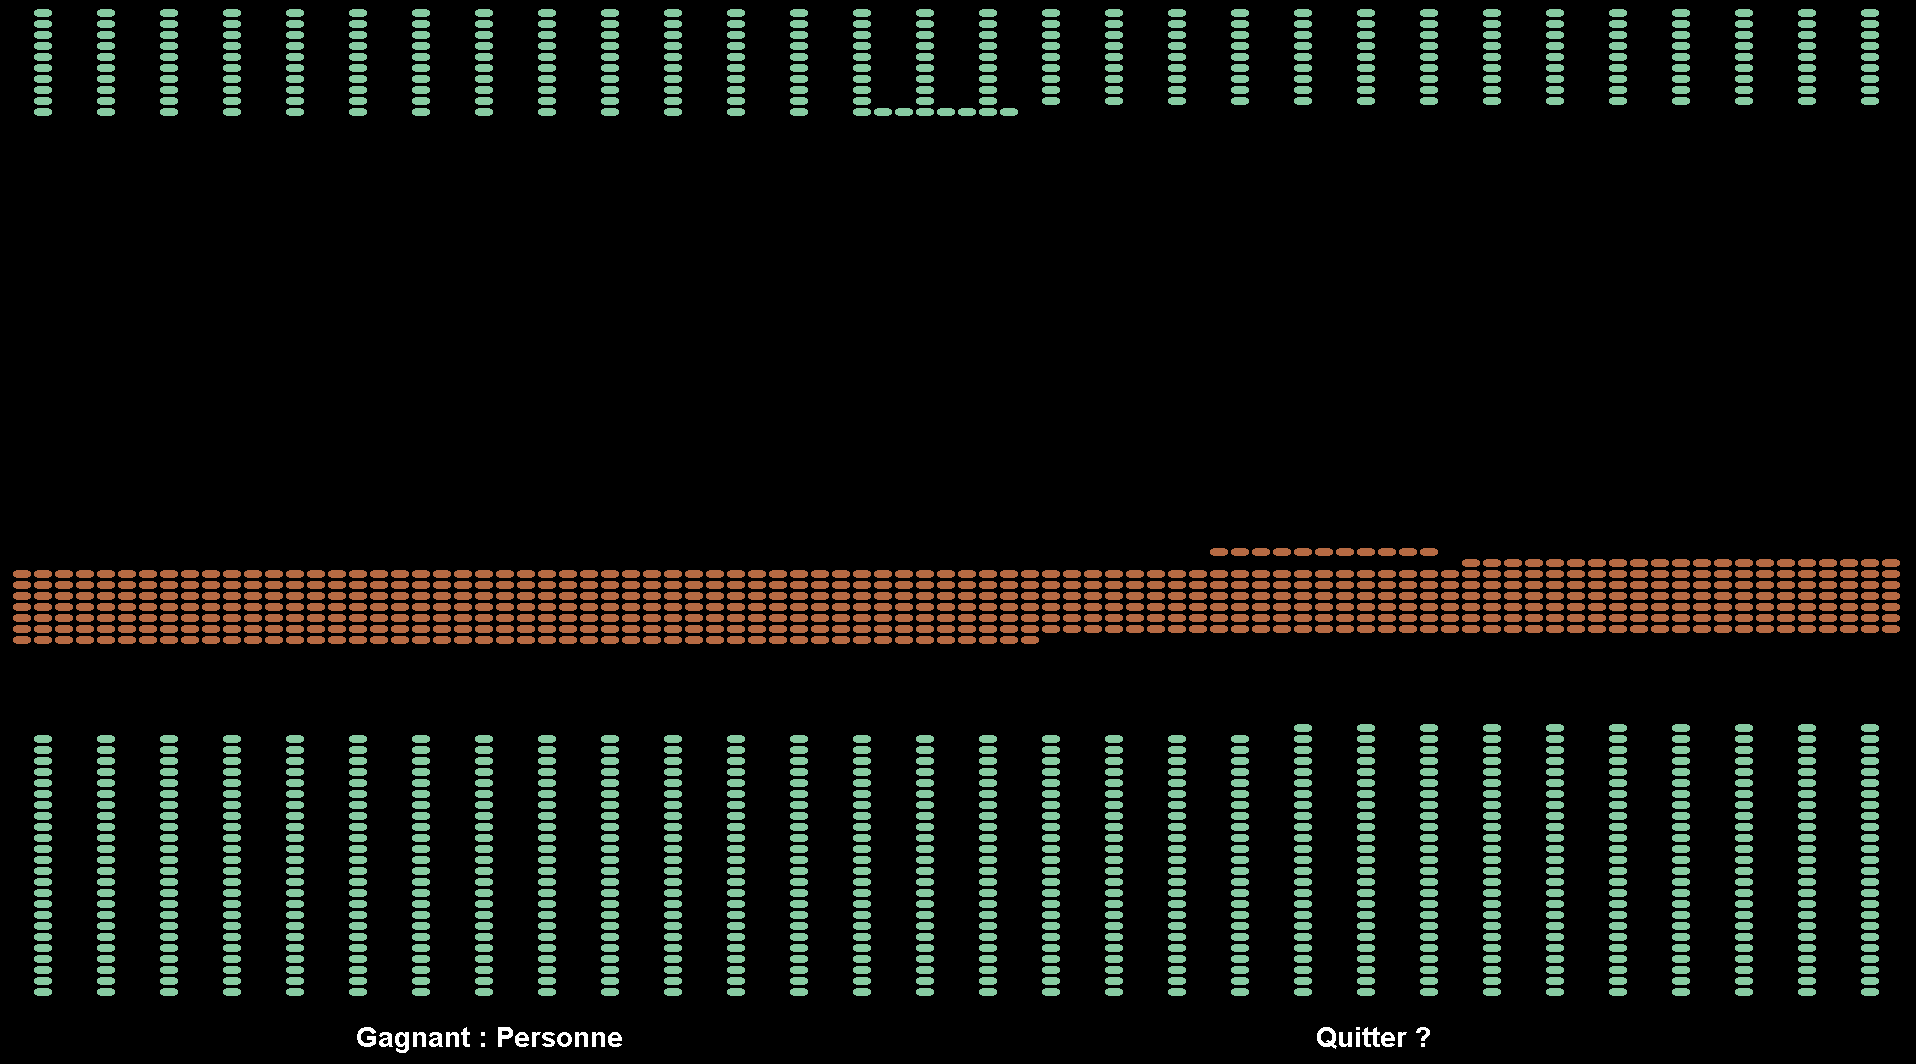
\includegraphics[scale=0.3]{cp.png}
\caption{exécution d'une partie entre deux warriors}
\end{figure}
Lors du démarrage d'une partie, deux couleurs sont choisies aléatoirement et définissent chacun un warrios différent. Il est possible de quitter la partie en cours en sélectionnant le bouton "quitter", ainsi qu'un affichage qui donnera le gagnant.
\section{Conclusion}
Aux vues du projet que nous avons crées, il semble évident que des améliorations sont possibles. Par exemple nous aurions pu trouver de meilleurs paramètres afin de générer des warriors encore plus performants. Aussi, nous aurions aimé intégrer un menu permettant entre autres de pouvoir écrire des warriors directement dans le programme ou encore un éditeur permettant de gérer les warriors. Néanmoins, nous avons su faire preuve d'organisation et de travail d'équipe afin de fournir un programme complet sans pour autant accabler l'un des membres de notre groupe sous une charge de travail trop lourde. Mais la chose la plus importante que ce projet nous a appris, c'est le fonctionnement des virus. En effet, les virus informatiques peuvent agir de la même façon afin d'infester un système. Un travail enrichissant et qui nous a montrés à quel point un si vieux jeu peut encore aujourd'hui regrouper une si grande communauté de passionnés dont nous faisons désormais partie intégrante.
\pagebreak
\section{Références}
\begin{enumerate}
\item 1987 first Half [en ligne] Disponible sur : \\
\href{http://para.inria.fr/~doligez/corewar/by-date/X1987first.htm}{http://para.inria.fr/~doligez/corewar/by-date/X1987first.html}

\item CoreWar [en ligne] Disponible sur : \\
\href{https://fr.wikipedia.org/wiki/Core_War}{https://fr.wikipedia.org/wiki/CoreWar}

\item C'est quoi les CoreWars ? [en ligne] Disponible sur : \\
\href{http://sebsauvage.net/comprendre/corewars/index.html}{http://sebsauvage.net/comprendre/corewars/index.html}

\item CoreWar [en ligne] Disponible sur : \\
\href{https://www.corewars.org/}{https://www.corewars.org/}

\item Nicolab [en ligne] Disponible sur : \\
\href{http://nicolab.chez.com/corewar/cw_docjeu.htm}{http://nicolab.chez.com/corewar/cwdocjeu.htm}

\item Championship [en ligne] Disponible sur : \\
\href{https://www.42.fr/corewar-championship-2017-dota-fauster/}{https://www.42.fr/corewar-championship-2017-dota-fauster/}

\item para [en ligne] Disponible sur : \\
\href{http://para.inria.fr/~doligez/corewar/}{http://para.inria.fr/~doligez/corewar/}

\item vxuser [en ligne] Disponible sur : \\
\href{http://vyznev.net/corewar/guide.html}{http://vyznev.net/corewar/guide.html}

\item The Redcode ICWS-88 standard [en ligne] Disponible sur : \\
\href{http://corewar.co.uk/standards/icws88.txt}{http://corewar.co.uk/standards/icws88.txt}
\end{enumerate}

\end{document}
